%
% 02_JPEG.tex
%
% (c) 2020 Prof Dr Andreas Müller, Hochschule Rapperswil
%
% !TEX root = ../../buch.tex
% !TEX encoding = UTF-8
%
\section{JPEG Kompression
\label{jpeg:section:kompjpeg}}
\rhead{JPEG Kompression}
Bei der JPEG Kompression nutzt man aus, dass Bilder kaum harte Übergänge bei Helligkeit und Farbe zeigen.
Diese Informationen kann man also ohne einen grossen Qualitätsverlust reduzieren. 

Um Bilder mit der DCT transformieren zu können, ist eine Vorverarbeitung nötig. 
Mit der Farbraumumrechnung erreicht man eine bessere Kompression.
Ausserdem wird das gesamte Bild in \(8\times8\) Pixelblöcke unterteilt, da die zweidimensionale DCT damit arbeitet.

\subsection{Farbraumumrechnung
\label{jpeg:subsection:farbraumumrechnung}}
Ein weit verbreitetes Farbmodell ist Rot-Grün-Blau (RGB), dabei wird eine Pixelfarbe mit einem Rot-, Grün- und Blauwert additiv erzeugt.
Das findet Anwendung bei allen Bildschirmen und fast allen Bildsensoren.

Beim JPEG-Standart wechselt man die Basis, in der die Farben dargestellt werden und benutzt statt RGB das YCbCr-Modell.
Dieses Modell teilt sich in die Komponenten Helligkeit (Luminanz Y) und Farbigkeit (Chrominanz) auf.
Die Chrominanz \(C_b\) steht für die Abweichung von Grau in Richtung Blau/Gelb und \(C_r\) für die Abweichung von Grau nach Rot/Türkis.

Das YCbCr-Modell wird angewandt, weil unsere Augen empfindlicher sind auf Helligkeitsunterschiede als auf Farbunterschiede.
Damit lassen sich, nach einer DCT, die Koeffizienten aus den \(C_b\) und \(C_r\) Bildblöcken stärker reduzieren als die in dem entsprechenden \(Y\) Block.
Der beschriebene Farbraumwechsel lässt sich mittels
\begin{equation}
    \begin{pmatrix}
        Y\\
        C_b\\
        C_r\\
    \end{pmatrix}
    \thickapprox
    \begin{pmatrix}
        0\\
        128\\
        128\\
    \end{pmatrix}
    +
    \begin{pmatrix*}[r]
        0.299\phantom{000} & 0.587\phantom{000} & 0.114\phantom{000}\\
        -0.168736 & -0.331264 & 0.5\phantom{00000}\\
        0.5\phantom{00000} & -0.418688 & -0.081312\\
    \end{pmatrix*}
    \cdot
    \begin{pmatrix}
        R\\
        G\\
        B\\
    \end{pmatrix}
    \label{jpeg:equation:farb}
\end{equation}
berechnen.
Durch begrenzte Rechengenauigkeit und Rundungsfehler entstehen hier erste Informationsverluste.

\subsection{Tiefpassfilter und Unterabtastung
\label{jpeg:subsection:tiefpass}}

\begin{figure}
    \centering
    \subfigure{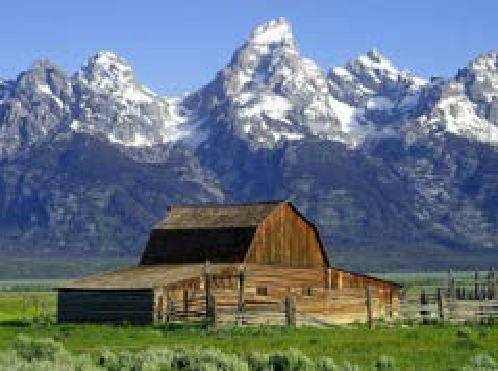
\includegraphics[width=0.43\textwidth]{papers/jpeg/pictures/rgb.pdf}}\qquad
    \subfigure{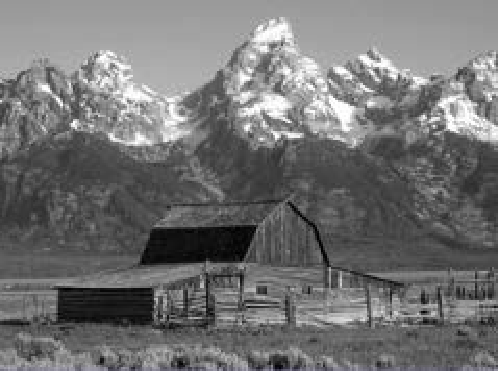
\includegraphics[width=0.43\textwidth]{papers/jpeg/pictures/y.pdf}}
    \vskip1ex
    \noindent
    \subfigure{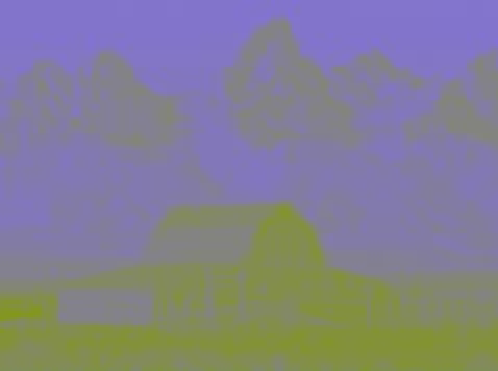
\includegraphics[width=0.43\textwidth]{papers/jpeg/pictures/cb.pdf}}\qquad
    \subfigure{
\includegraphics[width=0.43\textwidth]{papers/jpeg/pictures/cr.pdf}}
    \caption{Original, Luminanz (Y), Chrominanz Blau/Gelb (\(C_b\)) und Rot/Türkis (\(C_r\)) \label{jpeg:fig:ycbcr}}
\end{figure}


Im Abschnitt \ref{jpeg:subsection:farbraumumrechnung} wurde beschrieben, dass die Farbauflösung der \(C_b\) und \(C_r\) für Menschen deutlich geringer ist wie in Abb. \ref{jpeg:fig:ycbcr} ersichtlich.
Dazu werden sie Tiefpass gefiltert, zudem üblicherweise vertikal und horizontal um den Faktor 2 unterabgetastet, was einer vierfachen Datenreduktion entspricht.
Die Farbunterabtastung bedeutet, dass jeder Pixel des Bild seinen eigenen Helligkeitswert behält, wobei vier benachbarte Pixel sich die Farbinformationen teilen.

Beispiel: Beim \(8\times8\) Pixelblock der Luminanz hat jeder Pixel einen einzelnen Grauwert.
Bei den beiden Chrominanzen \(C_b\) und \(C_r\) werden jeweils \(2\times2\) Blöcke (innerhalb der \(8\times8\) Blöcke) den gleichen Wert zugewiesen.
Die Chrominanzen haben daher eine geringere Auflösung als die Luminanz.

\subsection{Tiling
\label{jpeg:subsection:tiling}}
Beim Tiling wird das Bild in Blöcke von jeweils \(8\times8\) Pixel unterteilt.
Da sich die Seitenlängen eines Bildes normalerweise nicht durch 8 teilen lassen, werden die restlichen Zeilen bzw. Spalten jeweils aufgefüllt.
Wie das Auffüllen geschieht, ist im JPEG-Standard nicht festgelegt.
Eine gängige Methode ist das Wiederholen der letzte Pixel-Zeile oder -Spalte bis es durch 8 teilbar ist, siehe Abb. \ref{jpeg:fig:tiling}.
Auf diese einzelnen Blöcke wird nun die DCT angewendet.

\begin{figure}
    \centering
    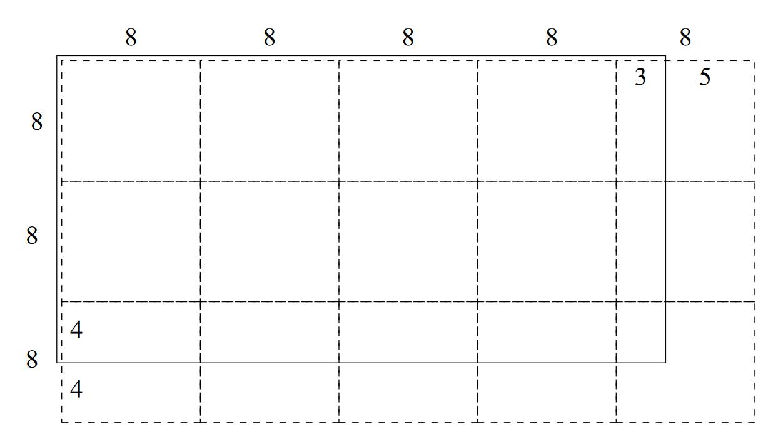
\includegraphics[width=120mm]{papers/jpeg/pictures/unterteilung.pdf}
    \caption{Bildeinteilung und Erweiterung
        \label{jpeg:fig:tiling}}
\end{figure}

\begin{table}[b]
    \centering
    \begin{tabular}{*{8}{r}}
        134.49 & 132.21 & 130.94 & 130.18 & 130.44 & 129.68 & 126.98 & 124.6\phantom{0}  \\
        137.73 & 137.73 & 138.85 & 139.71 & 138.73 & 134.44 & 127.84 & 122.32 \\
        148.5\phantom{0}  & 146.78 & 144.76 & 143.9\phantom{0}  & 142.36 & 137.31 & 131\phantom{.00}    & 126.14 \\
        155.37 & 150.22 & 143.14 & 138.57 & 136.55 & 135.79 & 133.58 & 132.72 \\
        153.04 & 148.47 & 141.88 & 138.08 & 135.54 & 134.78 & 132.79 & 131.07 \\
        146.95 & 145.43 & 144.16 & 142.64 & 140.86 & 136.3\phantom{0}  & 129.45 & 124.89 \\
        149.99 & 149.22 & 148.46 & 147.7\phantom{0}  & 144.74 & 138.07 & 129.47 & 123.85 \\
        160.7\phantom{0}  & 156.66 & 151.9\phantom{0}  & 147.7\phantom{0}  & 143.03 & 138.07 & 132.9\phantom{0}  & 128.61
    \end{tabular}
    \caption{Beispiel: Luminanzwerte eines \(8\times8\) Pixelblocks aus einem Bild.
        \label{jpeg:tab:orgblock}}
\end{table}

\subsection{Quantisierung
\label{jpeg:subsection:quantisierung}}
Bei allen verlustbehafteten Komprimierungsverfahren geschieht die eigentliche Datenreduktion erst bei der Quantisierung.
Dazu werden die Koeffizienten aus der DCT mit einer Quantisierungstabelle elementweise dividiert und auf den nächsten ganzzahligen Wert gerundet.
Die Quantisierungtabelle ist für die Qualität und Menge der reduzierten Daten verantwortlich.
Die Quantisierung erfolgt mittels: 
\begin{equation}
    F^Q(x,y)
    =
    \operatorname{round} \left(
    \frac{F(x,y)}{Q(x,y)}
    \right)
\end{equation}
dabei ist \(F^Q\) der resultierende Koeffizienten-Block, \(F\) ist der transformierte Pixelblock und \(Q\) die Quantisierungstabelle.
In Tabelle \ref{jpeg:tab:quantblock} sind die Werte des Beispielblocks quantisiert.

Bei diesem Schritt findet die Irrelevanzreduktion statt.
Irrelevanzreduktion meint, die Daten zu entfernen, die durch mathematische Modelle oder mittels empirischer Werte als irrelevant gekennzeichnet sind.
Beispiel: Personen mit Rot/Grün Blindheit erkennen kaum Unterschiede zwischen Rot und Grün, deshalb ist eine der beiden Farben irrelevant.
Es könnten daher entweder nur die Rot- oder nur die Grün-Anteile gespeichert werden.

Das Auge ist empfindlicher auf hohe Farbunterschiede von benachbarten Pixel, das sind die tiefen Frequenzen in der DCT Koeffizienten.
Daher werden diese weniger reduziert als die hohen Frequenzen, man sollte dafür eine optimale Tabelle verwenden.

Da der JPEG-Standard dies nicht vorgibt, muss die verwendete Tabelle im Header des Files mit abgelegt werden.
Tabelle \ref{jpeg:tab:quant} zeigt je eine gängige Quantisierungstabelle für die Luminanz und für die Chrominanzen.
Was auffällt ist, dass die Tabelle für die Luminanz aus \ref{jpeg:tab:quant} nicht symmetrisch ist.
Die Tabellen sind aus Untersuchungen des Sehverhaltens entwickelt worden, um Fehler so gering wie möglich zu halten und trotzdem eine gute Datenreduktion zu erzielen.

\begin{table}[t]
    \centering
    \begin{tabular}{*{8}{>{$}r<{$}}}
        1110.12 & 54.38  & -7.7\phantom{0}  & 9.19  & 0.3\phantom{0}   & 0.12  & 0.21  & -0.14 \\
        -27.43  & -15.67 & 0.12  & 0.19  & -0.19 & -0.02 & 0.09  & 0.18  \\
        -8.46   & -1.62  & -8.06 & -0.66 & -0.01 & 0.5\phantom{0}   & 0.08  & 0.43  \\
        -18.53  & -8.46  & -0.58 & -0.21 & -0.29 & -0.08 & 0.38  & 0\phantom{.00}    \\
        0.05    & 0.1\phantom{0}    & 15.43 & 0.02  & -0.13 & 0.31  & 0.07  & -0.35 \\
        -0.54   & -0.46  & 0.39  & 0.16  & 0.32  & -0.51 & 0.22  & 0.03  \\
        0.82    & 0.61   & 0.68  & 0.22  & 0.07  & -0.03 & 0.03  & 0.29  \\
        0.88    & 0.51   & -0.53 & 0.08  & 0.16  & 0.09  & -0.37 & -0.1\phantom{0} 
    \end{tabular}
    \caption{Beispiel: Tabelle \ref{jpeg:tab:orgblock} nach der DCT.
        \label{jpeg:tab:dctblock}}
\end{table}

\begin{table}[]
    \centering
    \begin{tabular}{*{8}{>{$}r<{$}}}
        69 & 5  & -1 & 1  & 0  & 0  & 0  & 0 \\
        -2 & -1 & 0  & 0  & 0 & 0 & 0  & 0  \\
        -1 & 0 & -1 & 0 & 0 & 0  & 0  & 0  \\
        -1 & 0 & 0 & 0 & 0 & 0 & 0  & 0 \\
        0  & 0  & 0  & 0  & 0 & 0  & 0  & 0 \\
        0 & 0 & 0  & 0  & 0  & 0 & 0  & 0  \\
        0  & 0  & 0  & 0  & 0  & 0 & 0  & 0  \\
        0  & 0  & 0 & 0  & 0  & 0  & 0 & 0
    \end{tabular}
     \caption{Beispiel: Tabelle \ref{jpeg:tab:dctblock} nach der Quantisierung.
        \label{jpeg:tab:quantblock}}
\end{table}

\begin{table}[b]
    \centering
    \begin{tabularx}{0.47\linewidth}{|X|X|X|X|X|X|X|X|}
        \hline
        16 & 11 & 10 & 16 & 24  & 40 & 51 & 61    \\ \hline
        12 & 12 & 14 & 19 & 26  & 58 & 60 & 55    \\ \hline
        14 & 13 & 16 & 24 & 40  & 57 & 69 & 56    \\ \hline
        14 & 17 & 22 & 29 & 51  & 87 & 80 & 62    \\ \hline
        18 & 22 & 37 & 56 & 68  & 109 & 103 & 77  \\ \hline
        24 & 35 & 55 & 64 & 81  & 104 & 113 & 92  \\ \hline
        49 & 64 & 78 & 87 & 103 & 121 & 120 & 101 \\ \hline
        72 & 72 & 95 & 98 & 112 & 100 & 103 & 99  \\ \hline        
    \end{tabularx}
    \qquad
    \begin{tabularx}{0.47\linewidth}{|X|X|X|X|X|X|X|X|}
        \hline
        17 & 18 & 24 & 47 & 99 & 99 & 99 & 99  \\ \hline
        18 & 21 & 26 & 66 & 99 & 99 & 99 & 99  \\ \hline
        24 & 26 & 56 & 99 & 99 & 99 & 99 & 99  \\ \hline
        47 & 66 & 99 & 99 & 99 & 99 & 99 & 99  \\ \hline
        99 & 99 & 99 & 99 & 99 & 99 & 99 & 99  \\ \hline
        99 & 99 & 99 & 99 & 99 & 99 & 99 & 99  \\ \hline
        99 & 99 & 99 & 99 & 99 & 99 & 99 & 99  \\ \hline
        99 & 99 & 99 & 99 & 99 & 99 & 99 & 99  \\ \hline  	  
    \end{tabularx}
    \caption{Beispiel Quantisierungstabelle für Luminanz (links) und Chominanzen (rechts).
        \label{jpeg:tab:quant}}
\end{table}



\subsection{Umsortierung und Differenzkodierung
\label{jpeg:subsection:umsortierung}}
Die 64 Koeffizienten des Pixelblocks Tabelle \ref{jpeg:tab:quantblock} werden nach der Quantisierung im Zig-Zag Muster abgetastet wie Abb. \ref{jpeg:fig:zigzag} zeigt, es resultiert
\begin{equation}
    69, 5, -2, -1, -1, -1, 1, 0, 0, -1, 0, 0, -1, 0, 0,\dots, 0.
    \label{jpeg:equation:abgetastet}
\end{equation}
Links oben ist der Gleichanteil (DC-Wert), der die mittlere Helligkeit des Blocks angibt.
Die restlichen Werte des Blocks nennt man den Wechselanteil (AC-Wert).
Der AC-Wert steigt im Verlauf des Zig-Zag und erreicht im letzten Wert die höchste Frequenz.

Die Koeffizienten mit hohem Wert (die niedrigen Frequenzen) stehen nun am Anfang, die Koeffizienten mit niedrigem Wert weiter hinten.
Je stärker quantisiert wurde, desto mehr Nullen sind am Ende der Zahlenfolge, das ist für eine Lauflängenkodierung optimal.

\begin{figure}
    \centering
    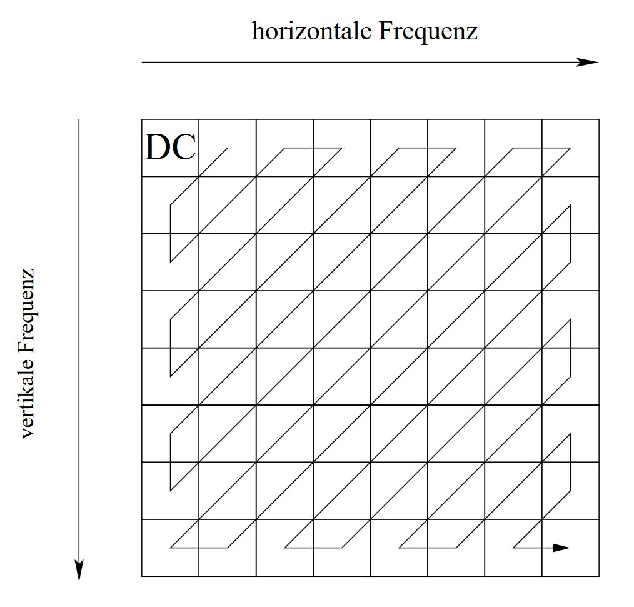
\includegraphics[width=75mm]{papers/jpeg/pictures/zigzag.pdf}
    \caption{Zig-Zag Abtastung der Koeffizienten
        \label{jpeg:fig:zigzag}}
\end{figure}

Der DC-Wert und die AC-Werte werden getrennt behandelt.
Der Grund dafür ist, dass Bilder oft grössere, fast gleichfarbige Flächen besitzen.
Dadurch haben benachbarte Blöcke ähnliche Gleichanteile, die differenziell kodiert werden.

Das bedeutet, man betrachtet nicht jeden DC-Wert einzeln, sondern die Differenzen zwischen den Blöcken.
Die Differenzkodierung beginnt mit dem zweiten Block des Bildes.
Durch die Differenzbildung wird der kodierte Wert kleiner, damit benötigt man weniger Bits.

Wenn an dem Beispiel in Tabelle \ref{jpeg:tab:quantblock} die differenzielle Kodierung angewendet wird, wird vom DC-Wert 69 der Wert des vorherigen Blocks (76) abgezogen \(69-76 = -7\).

\subsection{Entropiekodierung
\label{jpeg:subsection:entropiekodierung}}
Die Entropiekodierung der JPEG Kompression basiert auf dem Prinzip von David A. Huffman (Huffmancoding).
Bei der Entropiekodierung wird eine Zeichenfolge (z.B. aus einem Text) in eine Bitfolge umgewandelt.
Das geschieht mit Hilfe von Huffman-Trees.
Im Huffman-Tree wird die Häufigkeit der zu verschlüsselnden Werte berücksichtigt.
Werte die am meisten vorkommen erhalten dadurch kürzere Bitfolgen.
Die Huffman Kodierung zweigt beim Huffman-Tree von jedem Knoten nach links mit 0 und nach rechts mit 1 ab.
Um z.B. den Wert 4 zu erhalten, braucht man die Bitfolge 101.
Um den verschlüsselten Wert wieder zu dekodieren, muss man bei jedem Knoten entsprechend abzweigen, bis man im Huffman-Tree ein Ende erreicht. Beispiel: 1110 entspricht 6, in Abb. \ref{jpeg:fig:huffman} orange gekennzeichnet.

Der Huffman-Tree ist im JPEG-Standard nicht vorgegeben und muss deshalb im File header hinterlegt werden.
Dazu kommt, dass die binären Werte aus Tabelle \ref{jpeg:tab:huffman} alternativ kodiert werden können.

\begin{figure}[t]
    \centering
    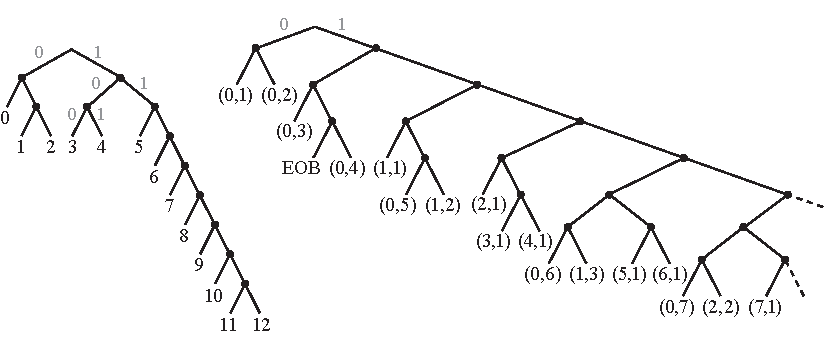
\includegraphics[width=\textwidth]{papers/jpeg/pictures/huffman.pdf}
    \caption{Beispiel für einen Huffman-Tree für den DC-Wert (links) \cite{jpeg:dccomponentyoutube} und die AC-Werte als Paar (rechts) \cite{jpeg:accomponentsyoutube}
        \label{jpeg:fig:huffman}}
\end{figure}

\subsubsection{Gleichanteil
\label{jpeg:subsubsection:gleichanteil}}
Der differenzkodierte Gleichanteil wird direkt mit einem Huffman-Tree kodiert.
In Abb. \ref{jpeg:fig:huffman} sind die Bäume dargestellt.

Nun kann man mit Hilfe der Tabelle \ref{jpeg:tab:huffman} und den Bäumen, den Bitstream für diesen Pixelblock erstellen.
Der DC-Wert \(-7\) hat laut Tabelle \ref{jpeg:tab:huffman} die binäre Länge 3.
Aus dem Baum links gemäss Abb. \ref{jpeg:fig:huffman} ergibt sich dafür 100.
Aus der Tabelle \ref{jpeg:tab:huffman} liest man für den Wert \(-7\) den binären Wert 000.
Die binäre Länge 100 und der binäre Wert von \(-7\) mit 000 wird zusammen als 100000 geschrieben.

\subsubsection{Wechselanteil
\label{jpeg:subsubsection:wechselanteil}}
Um Speicherplatz zu reduzieren, werden die AC-Werte zuerst einer run length coding (RLC) unterzogen, dabei werden nur die Nullen berücksichtigt. 
Die kodierten Werte verschlüsselt ein Huffman-Tree anschliessend.

Die RLC der Wechselanteile erfolgt in einer Klammer-Sortierung.
Jede eckige Klammer steht für einen Wechselanteil aus \eqref{jpeg:equation:abgetastet}.
Der erste Wert in der runden Klammer gibt an, wie viele AC-Werte vor dem zu kodierenden Wert gleich Null sind.
Der zweite Wert in der runden Klammer die Anzahl der benötigten Bits für die Kodierung (s. Tabelle \ref{jpeg:tab:huffman}).
Darauf folgt der eigentliche AC-Wert selbst.
Aus den Wechselanteilen von \eqref{jpeg:equation:abgetastet} wird:
\begin{equation}
    [(0,3)5],[(0,2)-2],[(0,1)-1],\dots,[(2,1)-1], EOB.
    \label{jpeg:equation:kette}
\end{equation}
Nach dem letzten Wert \(\neq 0\) wird anstelle aller Null Einträge, als Abschluss der End-of-Block (EOB) hinzugefügt, der als (0,0) definiert ist.
Die runden Klammern, aus der zur Kette \eqref{jpeg:equation:kette} gepackten AC-Werte,  werden mit dem Baum gemäss Abb. \ref{jpeg:fig:huffman} in Bits umgewandelt.

Beispiel: Der Klammerausdurck \([(0,3)5]\) am Anfang der Kette in \eqref{jpeg:equation:kette} hat aus dem Baum den Wert 100 und die 5 gemäss Tabelle \ref{jpeg:tab:huffman} als binären Wert 101, was 100101 ergibt.
Werden alle Werte der Kette \eqref{jpeg:equation:kette} so verarbeitet, erhält man
\begin{equation}
    100000'100101'0101'000'000'000'001'111000'111000'1010    
\end{equation}
als Bitstream.
Die ersten 6 Bits sind aus dem DC-Wert, der Rest aus dem AC-Teil.

Der Bitstream besteht aus 44 Bits.
Hätte man die Werte aus Tabelle \ref{jpeg:tab:quantblock} genommen, bräuchte man \(8\times8\times8=512\) Bits, aus \(8\times8\) Einträgen mit jeweils 8 Bit Länge, was dem 11-fachen entspricht.

\begin{table}[b]
    \centering
    \begin{tabular}{l>{$}c<{$}l}
        Länge  & \textrm{Eintrag}                     & Binär\\
        0      & 0                           		  & \(-\) \\
        1      & -1,1                         	 	  & 0,1 \\
        2      & -3,-2,2,3                   		  & 00,01,10,11 \\
        3      & -7,-6,-5,-4,4,5,6,7         		  & 000,001,010,011,100,101,110,111 \\
        4      & -15,-14,\dots,-8,8,\dots,15          & 0000,0001,\dots,0111,1000,\dots,1111 \\
        5      & \dots                                & \dots \\
        6      & \dots                                & \dots \\
        \vdots & \vdots                               & \vdots \\
        12     & -4095,\dots,-2048,2048,\dots,4095    & \dots
    \end{tabular}
    \caption{Beispiel für eine Kodierung der Binären-Werte
        \label{jpeg:tab:huffman}}
\end{table}

\subsubsection{Beispiel zur Herleitung der Entropiekodierung
\label{jpeg:subsubsection:kodierung}}
\kreis{1} Kodierung eines Wechselanteils:
\begin{equation}
    \text{[(Anzahl Nullen,Bitlänge)Wert]}\nonumber
\end{equation}
das heisst der Wechselanteil von \eqref{jpeg:equation:abgetastet} hat die Kodierung
\begin{align}
    &[(0,?)5],[(0,?)-2],[(0,?)-1],[(0,?)-1],\\
    &[(0,?)-1],[(0,?)1],[(2,?)-1],[(2,?)-1],[(0,0)]\nonumber
\end{align}
\textcolor{RoyalBlue}{\kreis{2} ? aus Tabelle \ref{jpeg:tab:huffman} ergänzen:}
\begin{align}
    &[(0,\mathcolor{RoyalBlue}{3})5],[(0,\textcolor{RoyalBlue}{2})-2],[(0,\textcolor{RoyalBlue}{1})-1],[(0,\textcolor{RoyalBlue}{1})-1],\\
    &[(0,\textcolor{RoyalBlue}{1})-1],[(0,\textcolor{RoyalBlue}{1})1],[(2,\textcolor{RoyalBlue}{1})-1],[(2,\textcolor{RoyalBlue}{1})-1],[(0,0)]\nonumber
\end{align}
\textcolor{YellowOrange}{\kreis{3} Werte mit Hilfe Tabelle \ref{jpeg:tab:huffman} ins Binäre übersetzen:}
\begin{align}
    &[(0,\mathcolor{RoyalBlue}{3})\mathcolor{YellowOrange}{101}],[(0,\textcolor{RoyalBlue}{2})\mathcolor{YellowOrange}{01}],[(0,\textcolor{RoyalBlue}{1})\mathcolor{YellowOrange}{0}],[(0,\textcolor{RoyalBlue}{1})\mathcolor{YellowOrange}{0}],\\
    &[(0,\textcolor{RoyalBlue}{1})\mathcolor{YellowOrange}{0}],[(0,\textcolor{RoyalBlue}{1})\mathcolor{YellowOrange}{1}],[(2,\textcolor{RoyalBlue}{1})\mathcolor{YellowOrange}{0}],[(2,\textcolor{RoyalBlue}{1})\mathcolor{YellowOrange}{0}],[(0,0)]\nonumber
\end{align}
\textcolor{ForestGreen}{\kreis{4} Runde Klammern werden mit Huffman-Tree kodiert:}
\begin{align}
    &[\mathcolor{ForestGreen}{100}\mathcolor{YellowOrange}{101}],[\mathcolor{ForestGreen}{01}\mathcolor{YellowOrange}{01}],[\mathcolor{ForestGreen}{00}\mathcolor{YellowOrange}{0}],[\mathcolor{ForestGreen}{00}\mathcolor{YellowOrange}{0}],\\
    &[\mathcolor{ForestGreen}{00}\mathcolor{YellowOrange}{0}],[\mathcolor{ForestGreen}{00}\mathcolor{YellowOrange}{1}],[\mathcolor{ForestGreen}{11100}\mathcolor{YellowOrange}{0}],[\mathcolor{ForestGreen}{11100}\mathcolor{YellowOrange}{0}],[\mathcolor{ForestGreen}{1010}]\nonumber
\end{align}

\subsection{Probleme JPEG
\label{jpeg:subsection:probleme}}
Wenn man ein Bild zu stark komprimiert, treten Artefakte auf.
Artefakte zeigen sich bei Bildern als kleine Klötzchen, in Abb. \ref{jpeg:fig:blockart} deutlich erkennbar.
Die Ursache dafür ist das zu starke Quantisieren der \(8\times8\) Pixelblöcke nach der DCT.
Dadurch gehen zu viele Informationen verloren und der gesamte Block besitzt dieselbe Farbe.

Aus diesem Grund ist der JPEG-Standard ungeeignet für die Kompression von Texten und Fingerabdrücken.
Texte und Fingerabdrücke haben typischerweise harte Pixelübergänge.
Für die eindeutige Erkennung eines Fingerabdrucks darf seine Struktur nicht verändert werden.
Für diese beiden Anwendungen trifft die Annahme, die in Abschnitt \ref{jpeg:section:kompjpeg} über Bilder gemacht wurde nicht mehr zu.

Die Abb. \ref{jpeg:fig:textart} zeigt, was mit komprimiertem Text passiert.
Bei Abb. \ref{jpeg:fig:fingerprint} ist die linke Hälfte unkomprimiert und die rechte im JPEG-Format komprimiert.
Die Übertragung von JPEG ist anfällig auf Störungen.
Wird ein Bit des vom Huffman-Codierer erzeugten Datenstroms verfälscht, erhalten alle folgenden Bits eine andere Bedeutung. 
Dadurch kann ein falscher Bit das gesamte Bild verändern und unbrauchbar machen.



\begin{figure}[h]
    \centering
    \subfigure[Blockartefakte\label{jpeg:fig:blockart}]{
        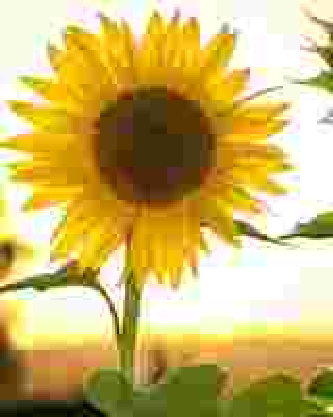
\includegraphics[width=0.32\textwidth]{papers/jpeg/pictures/sonnenblume.pdf}}
    \hfill
    \subfigure[Textartefakt\label{jpeg:fig:textart}]{
        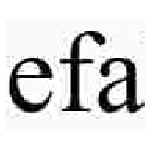
\includegraphics[width=0.34\textwidth]{papers/jpeg/pictures/artifakte.pdf}}
    \hfill
    \subfigure[Fingerprint\label{jpeg:fig:fingerprint}]{
        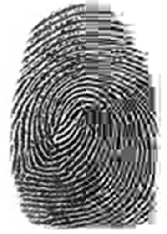
\includegraphics[width=0.28\textwidth]{papers/jpeg/pictures/fingerprint.pdf}}
    \caption{Verschiedene Artefakte von JPEG 
    \label{jpeg:fig:bspproblem}}
\end{figure}
